\documentclass[11pt,a4paper]{article}
\usepackage[T1]{fontenc}
\usepackage[utf8]{inputenc}
\usepackage{lmodern}
\usepackage[margin=2.5cm]{geometry}
\usepackage{amsmath,amssymb}
\usepackage{booktabs}
\usepackage{graphicx}
\usepackage[hidelinks]{hyperref}
\hypersetup{pdfauthor={Gianni Pilotti},pdftitle={Delta Hedging a Binary Option with a Perpetual},pdfcreator={},pdfproducer={}}
\setlength{\parindent}{0pt}
\setlength{\parskip}{6pt}

\title{Delta Hedging a Binary Option with a Perpetual}
\author{Gianni Pilotti}
\date{}

\begin{document}
\maketitle

\section{The Core Idea}

A ``Bitcoin above $K$'' binary pays \$1 if BTC settles above $K$ and nothing otherwise. The repository buys these contracts on Polymarket and hedges the BTC exposure with the Hyperliquid perpetual. The question is what the hedge costs and how much risk it removes.

\begin{itemize}
\item \textbf{Delta explodes near expiry:} a binary has a gamma that grows as $1/T$, so the hedge needs ever larger corrections close to settlement.
\item \textbf{Costs decide the result:} each rebalance pays the taker fee and the spread, so a hedge that tracks delta closely can lose more than a hedge that tracks it loosely.
\end{itemize}

The same hedge is then applied to a strip of Kalshi binaries and compared with Deribit options over 207 daily expiries (2026-03-19 to 2026-10-11).

\section{Method}

\subsection{Pricing and Greeks}

With zero rate, the code (\texttt{core/math\_engine.py}) prices the binary as a cash-or-nothing call:
\begin{equation}
d_2=\frac{\ln(S/K)-\tfrac12\sigma^2T}{\sigma\sqrt T},\qquad V=N(d_2),
\end{equation}
\begin{equation}
\Delta=\frac{\varphi(d_2)}{S\sigma\sqrt T},\qquad
\Gamma=-\frac{\varphi(d_2)\,d_1}{S^2\sigma^2T},\quad d_1=d_2+\sigma\sqrt T .
\end{equation}
$T$ is measured in years of 365 days. The implied volatility is the root of $N(d_2(\sigma))=V$. For $S<K$ the price peaks at $N(-\sqrt{2|\ln(S/K)|})<0.5$, so the code keeps the low-volatility root and returns nothing above that peak.

\subsection{Volatility Input}

The engine takes $\sigma$ from one of three sources: the volatility implied by the Polymarket mid, the Deribit DVOL index, or a time-weighted EWMA of Hyperliquid returns. The last valid implied value is held for 300 s, then the engine falls back to DVOL.

\subsection{Hedge Rules}

For $Q$ YES shares held, the target perp position in BTC is
\begin{equation}
h=-Q\,\Delta(S,K,\sigma,T).
\end{equation}
Two strategies are compared:
\begin{itemize}
\item \textbf{Static:} one limit order on the passive side of the Hyperliquid book, sized to the initial $h_0$. It is a maker order and fills only when a trade crosses its price.
\item \textbf{Dynamic:} a market order whenever $|h-\text{position}|$ exceeds $\max\!\big(\text{lot},\,\text{min notional}/S\big)$. With a \$10 minimum notional this threshold is about $1.2\times10^{-4}$ BTC, so small delta moves trigger orders.
\end{itemize}
A kill switch closes all positions at expiry minus 2 hours, before the gamma region.

\subsection{Execution and Fees}

Taker orders walk the order book level by level. There is no persistent market impact. Fees are those in \texttt{risk/fees.py}:
\begin{equation}
\text{fee}_{HL}=|N|\cdot b/10^4,\quad b=4.5\ (\text{taker}),\ 1.5\ (\text{maker}),
\qquad
\text{fee}_{PM}=C\cdot 0.07\cdot p(1-p).
\end{equation}
Here $N$ is the trade notional, $C$ the number of shares and $p$ the share price. The Polymarket maker fee is set to zero and the maker rebate is not modelled.

\subsection{Kalshi Strip}

A single Kalshi NO binary has the same exploding gamma. The strip buys NO contracts on 9 strikes spaced \$250 apart, with equal weights and the same premium budget as the single strike. Its payoff is a staircase that approximates a put spread of slope $n/250$ BTC per dollar, where $n$ is the number of contracts per leg. The delta of the strip is the sum of the NO deltas, so the gamma is spread over nine strikes instead of one.

\section{Results}

\subsection{Live Session}

The recorded session of 12 October 2026 lasted 41 minutes ($K=\$84{,}000$, $Q=1000$ shares). Amounts are in dollars.

\begin{center}
\begin{tabular}{lrrrrrr}
\toprule
Strategy & PM P\&L & HL P\&L & PM fees & HL fees & Funding & Total \\
\midrule
Static  & $-141.22$ & $+82.44$ & 16.05 & 5.70   & $-0.37$ & $-80.17$ \\
Dynamic & $-141.22$ & $+78.41$ & 16.05 & 127.76 & $-0.34$ & $-206.28$ \\
\bottomrule
\end{tabular}
\end{center}

The perp P\&L is similar in both cases. The gap of about \$122 in Hyperliquid fees comes from taker fees on the dynamic hedge.

\subsection{Single Strike, Strip and Deribit Options}

Hedged P\&L per daily expiry, net of Kalshi fees, Hyperliquid fees and funding. $\sigma$ is the DVOL value.

\begin{center}
\begin{tabular}{lrrr}
\toprule
Structure & Mean (\$) & Std (\$) & Winning days (\%) \\
\midrule
Kalshi single strike & $-85.01$ & 361.80 & 41.1 \\
Kalshi strip         & $-57.98$ & 185.95 & 31.9 \\
Deribit put spread   & $-36.3$  & 133.0  & 25.1 \\
Deribit vanilla put  & $-42.9$  & 175.9  & 27.1 \\
\bottomrule
\end{tabular}
\end{center}

\begin{itemize}
\item \textbf{Risk:} the strip cuts the standard deviation of daily P\&L by about half (ratio 0.514).
\item \textbf{Mean:} the strip improves the mean by \$27.03 per day, but the paired test gives $p=0.136$. This is not a significant gain.
\item \textbf{Deribit:} the put spread beats the strip by \$21.7 per day ($p=0.002$). The sign reverses in September--October ($-34.5$ per day) when the Kalshi spread narrows.
\end{itemize}

\begin{figure}[ht]
\centering
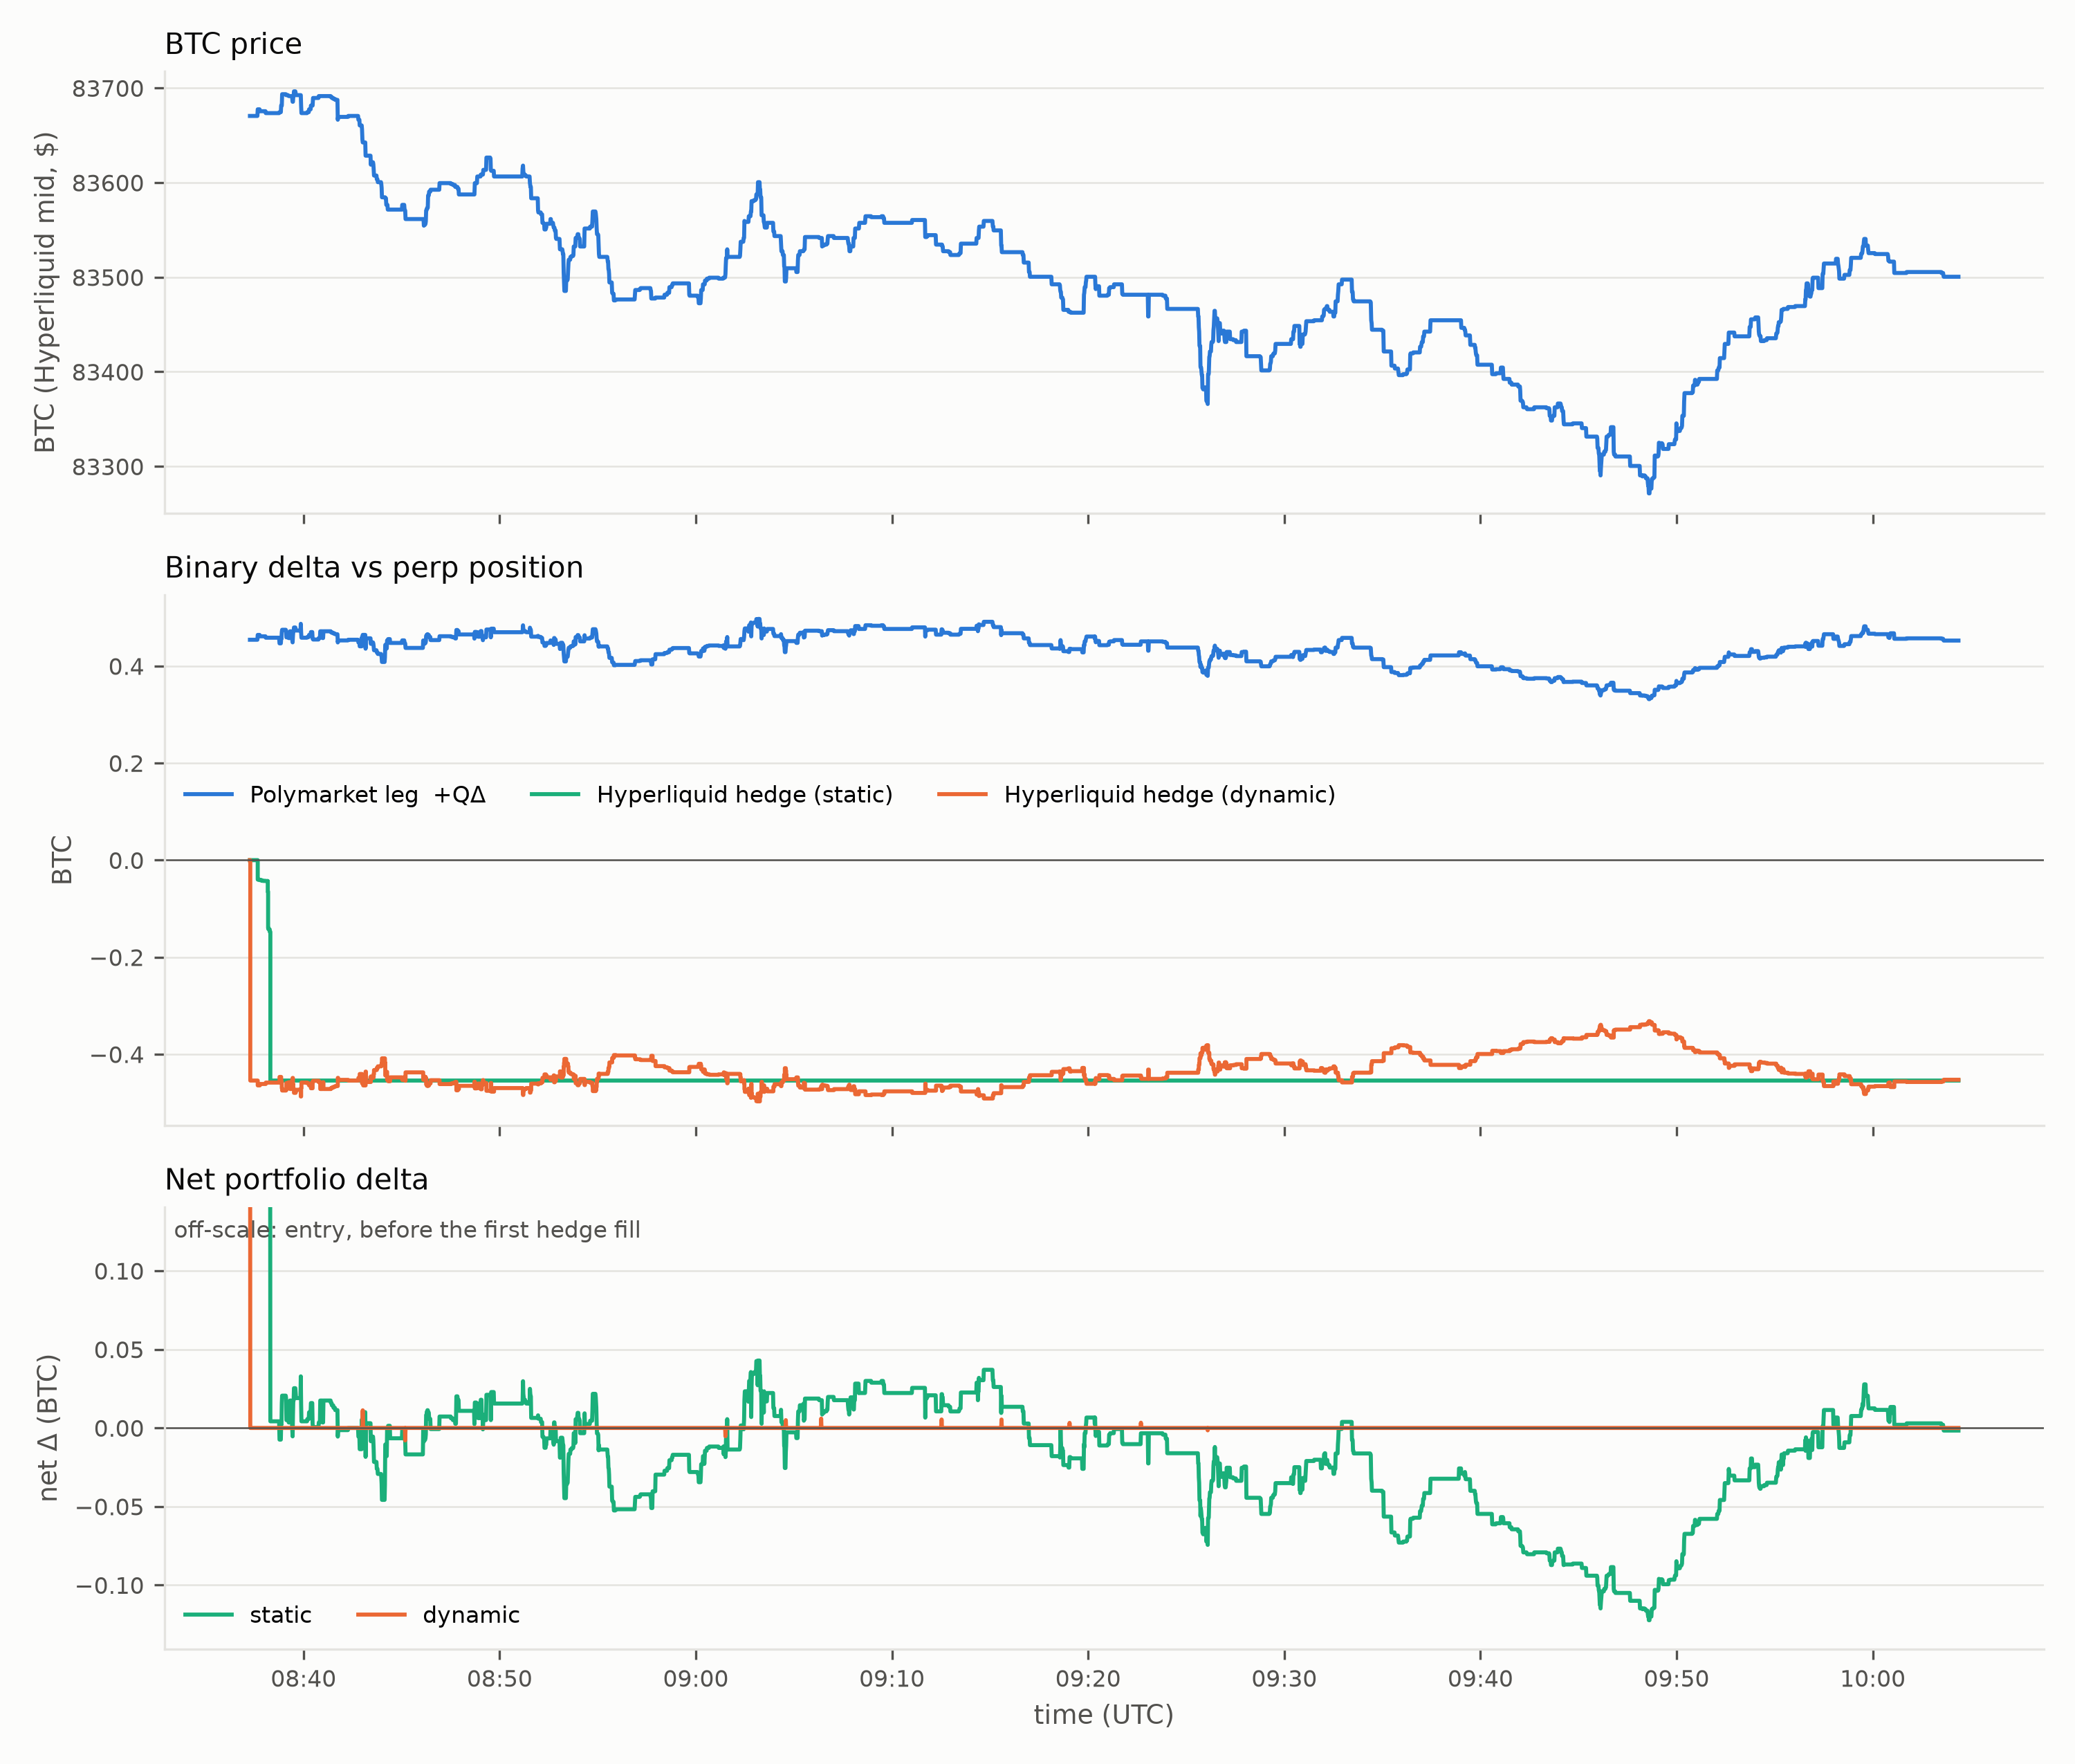
\includegraphics[width=0.92\textwidth]{../reports/hedge.png}
\caption{Live session: BTC price, binary delta against the two hedges, and net delta.}
\end{figure}

\section{Worked Example}

The inputs are illustrative: $S=83{,}600$, $K=84{,}000$, $\sigma=0.40$, $T=6$ hours, $Q=1000$ shares.

\textbf{Step 1.} $T=6\cdot3600/(365\cdot24\cdot3600)=6.849\times10^{-4}$ years, so $\sigma\sqrt T=0.010468$.

\textbf{Step 2.} $d_2=\big(\ln(83600/84000)-\tfrac12\cdot0.010468^2\big)/0.010468=-0.4612$, and $V=N(-0.4612)=0.3223$.

\textbf{Step 3.} $\Delta=\varphi(-0.4612)/(83600\cdot0.010468)=4.0986\times10^{-4}$ per share. The target hedge is $h=-1000\cdot\Delta=-0.4099$ BTC, a short of about \$34{,}264.

\textbf{Step 4.} At the taker fee the entry costs $34{,}264\cdot4.5/10^4=\$15.42$. As a maker order the fee is $34{,}264\cdot1.5/10^4=\$5.14$.

\textbf{Step 5.} If $S$ moves to 83,700, the delta becomes $0.4287$ BTC. The dynamic hedge sells another $0.01884$ BTC (\$1{,}577), which costs \$0.71 in taker fees. The first-order gamma estimate is $\Gamma\cdot Q\cdot100=0.0211$ BTC, slightly above the exact change.

One such rebalance is cheap. The cost of the dynamic hedge comes from the number of rebalances, not from their size.

\section{Limits}

\begin{itemize}
\item \textbf{One live session:} the static against dynamic comparison rests on 41 minutes of recorded data. The kill-switch checks that need the session to reach expiry are pending.
\item \textbf{Simulated fills:} the book is replayed as published, with no market impact. Large orders would fill worse.
\item \textbf{Maker fills:} a static limit order may not fill at all in real trading. The simulator fills it only when a trade crosses its price.
\item \textbf{Model risk:} the digital price depends on $\sigma$, and for $S<K$ the implied volatility has no root when the mid is above the price peak.
\item \textbf{Negative mean:} every structure loses on average after fees. These are backtest outputs over seven months, not a trading recommendation.
\end{itemize}

\end{document}
